% -*- root: ../gvoysey-thesis.tex -*-
\chapter{Results}
\label{chapter:Results}
\thispagestyle{myheadings}

% set this to the location of the figures for this chapter. it may
% also want to be ../Figures/2_Body/ or something. make sure that
% it has a trailing directory separator (i.e., '/')!
\graphicspath{{5_Results/Figures/}}
\section{Chapter Summary} % (fold)
\label{sec:results_summary}
This chapter describes the results obtained when using the modeling environment described in~\autoref{chapter:Methods} to simulate a series of tone-in-noise experiments performed in humans by \citeauthor{Mehraei2016Auditory} to elucidate certain aspects of cochlear synaptopathy. 

% section results_summary (end)
\section{Tone in noise} % (fold)
\label{sec:tone_in_noise}


\section{Simulations}
The experiment design tool described in \autoref{sec:automated_parameter_exploration} was used to specify a range of values for each parameter in Corti to reveal the relative contributions of each. 

\subsection{Stimuli} % (fold)
\label{sub:stimuli}
Following \citeauthor{Mehraei2015Auditory,Mehraei2016Auditory}, 6 stimului were programmatically generated and stored as WAV files with a sampling frequency of 100 kHz.  As shown in \autoref{fig:stimuli-used}, stimulus onset was delayed by 20 $\mu$s of silence, and then consisted of 80 dB SPL clicks with a repetition rate of 100 ms in the presence of gaussian noise at different signal to noise ratios. 

\begin{figure}[htbp]
	\centering
	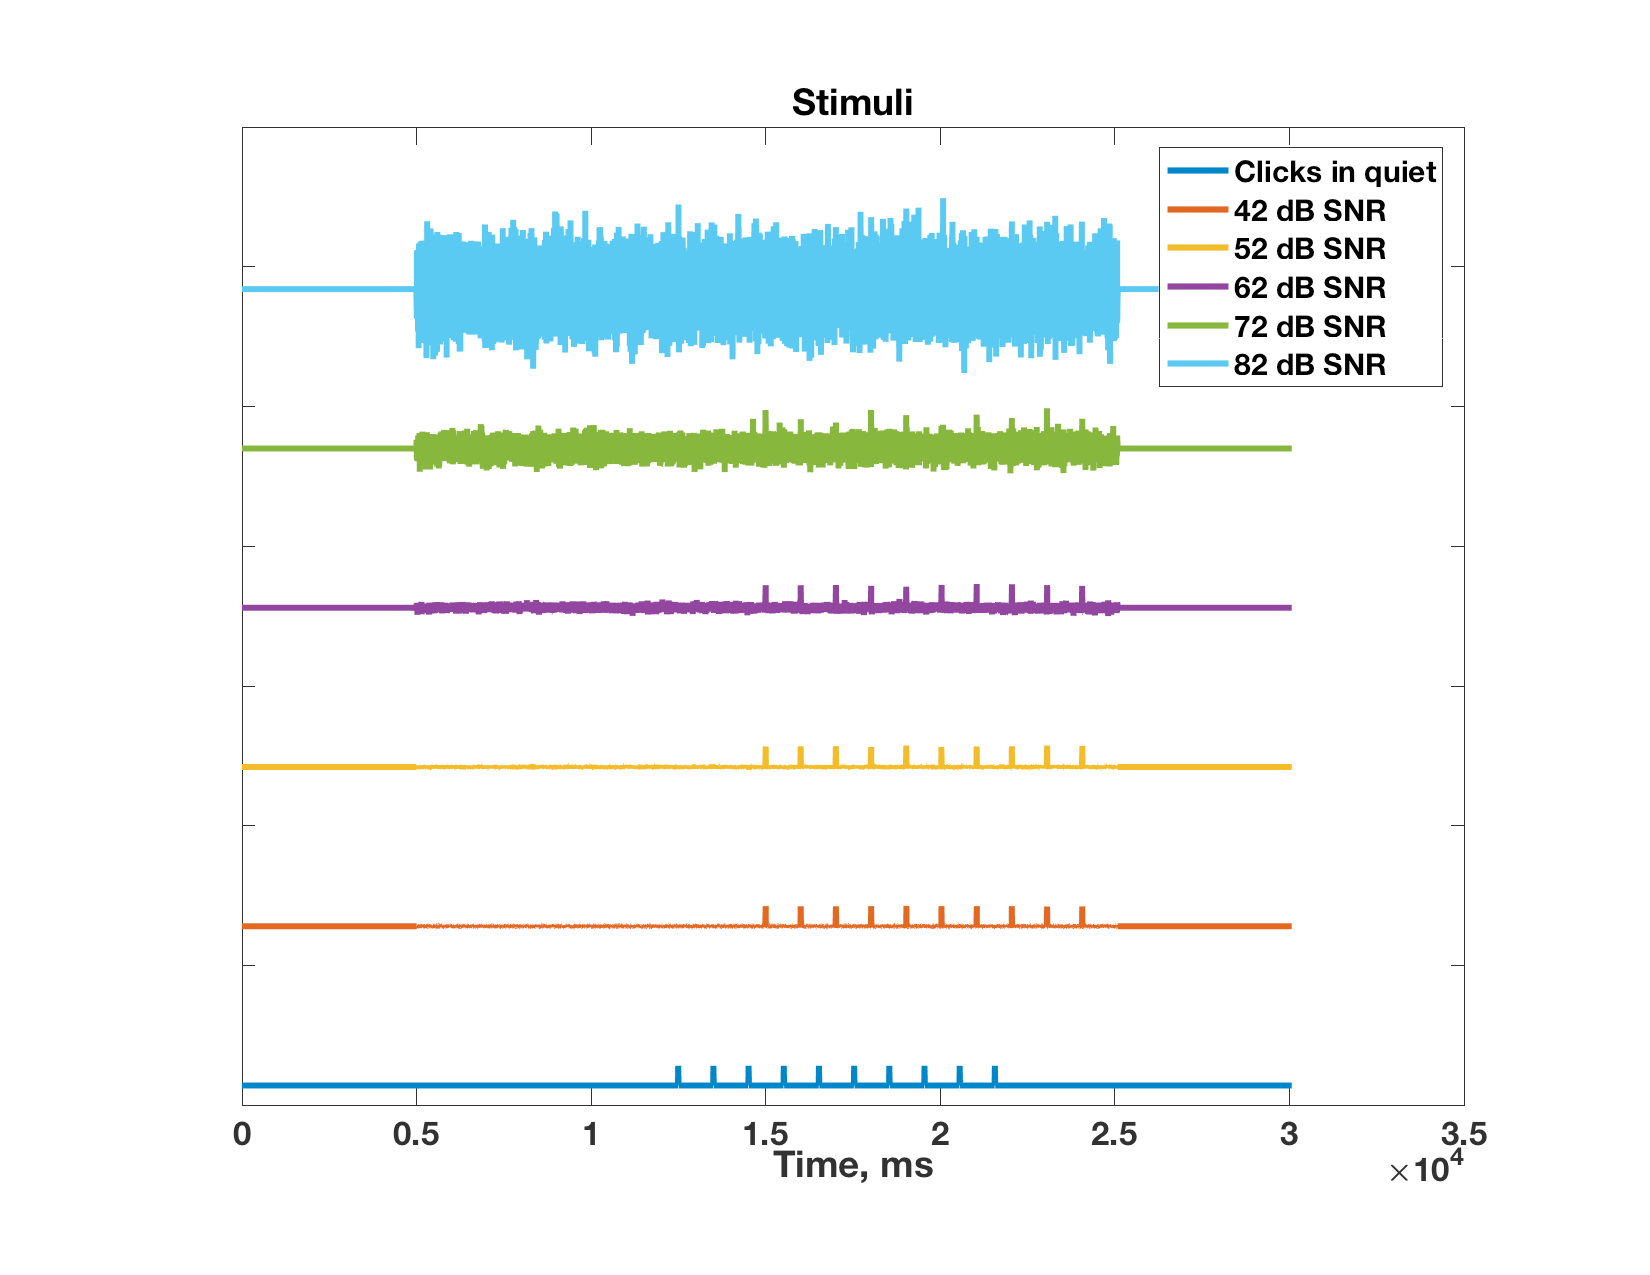
\includegraphics[width=0.95\textwidth]{stimuli-used.pdf}
	\caption[Experimental Stimuli]{Stimuli used to drive the auditory models.}
	\label{fig:stimuli-used}
\end{figure}

All other parameters--choice of peripheral and brainstem model and logistically weighted fiber distributions---were fully explored.

In total, 240 separate simulations were run in parallel on Boston University's high-performance computing cluster over the course of approximately 9 days.  Model output was automatically stored into a HDF5 database approximately 250 GB in size.


\section{Effect of Synaptopathy} % (fold)
\label{sec:effect_of_synaptopathy}
The effects of four types of synaptopathy---moderate, severe, low-SR specific moderate, and low-SR specific severe---were simulated, with the synaptic degradation parameters as given in \autoref{fig:synaptopathy}. 

\begin{figure}[htbp]
	\centering
	\includegraphics[page=5,width=0.95\textwidth]{wave1and5.pdf}
	\caption[Effects of Synaptopathy]{The effects of varying levels of synaptopathy on model responses to a stimulus at multiple noise levels.  Some traces (top) are present but not visible as they precisely overlay other results.}
	\label{fig:wave1results}
\end{figure}

The effect of fiber loss on Wave V peak latency and Wave 1 peak amplitude are given in \autoref{fig:wave1results}.  Consistent with prediction, Wave I amplitudes are decreased as a function of synaptopathy, as well as a function of increasing noise masker level.  Wave V latencies exhibit a decrease in latency but only for some masker levels.  
% section effect_of_synaptopathy (end)

\section{Effect of peripheral model} % (fold)
\label{sec:effect_of_peripheral_model}
The verhulst and zilany models will produce different estimates of the auditory nerve response. Prior work had their results very different; with recent changes to the verhulst model, this may have changed.
% section effect_of_peripheral_model (end)


\section{Effect of CF weighting} % (fold)
\label{sec:effect_of_cf_weighting}
In models of the periphery that include more low SR fibers at high frequencies, synaptopathic losses will change.
% section effect_of_cf_weighting (end)

\section{Effect of brainstem model} % (fold)
\label{sec:effect_of_brainstem_model}
Does our intuition about a more physiologicaly relevant brainstem and midbrain model capturing more of the diversity of human responses bear out? 
% section effect_of_brainstem_model (end)